% GNUPLOT: LaTeX picture with Postscript
\begingroup
  % Encoding inside the plot.  In the header of your document, this encoding
  % should to defined, e.g., by using
  % \usepackage[cp1252,<other encodings>]{inputenc}
  \inputencoding{cp1252}%
  \makeatletter
  \providecommand\color[2][]{%
    \GenericError{(gnuplot) \space\space\space\@spaces}{%
      Package color not loaded in conjunction with
      terminal option `colourtext'%
    }{See the gnuplot documentation for explanation.%
    }{Either use 'blacktext' in gnuplot or load the package
      color.sty in LaTeX.}%
    \renewcommand\color[2][]{}%
  }%
  \providecommand\includegraphics[2][]{%
    \GenericError{(gnuplot) \space\space\space\@spaces}{%
      Package graphicx or graphics not loaded%
    }{See the gnuplot documentation for explanation.%
    }{The gnuplot epslatex terminal needs graphicx.sty or graphics.sty.}%
    \renewcommand\includegraphics[2][]{}%
  }%
  \providecommand\rotatebox[2]{#2}%
  \@ifundefined{ifGPcolor}{%
    \newif\ifGPcolor
    \GPcolortrue
  }{}%
  \@ifundefined{ifGPblacktext}{%
    \newif\ifGPblacktext
    \GPblacktextfalse
  }{}%
  % define a \g@addto@macro without @ in the name:
  \let\gplgaddtomacro\g@addto@macro
  % define empty templates for all commands taking text:
  \gdef\gplbacktext{}%
  \gdef\gplfronttext{}%
  \makeatother
  \ifGPblacktext
    % no textcolor at all
    \def\colorrgb#1{}%
    \def\colorgray#1{}%
  \else
    % gray or color?
    \ifGPcolor
      \def\colorrgb#1{\color[rgb]{#1}}%
      \def\colorgray#1{\color[gray]{#1}}%
      \expandafter\def\csname LTw\endcsname{\color{white}}%
      \expandafter\def\csname LTb\endcsname{\color{black}}%
      \expandafter\def\csname LTa\endcsname{\color{black}}%
      \expandafter\def\csname LT0\endcsname{\color[rgb]{1,0,0}}%
      \expandafter\def\csname LT1\endcsname{\color[rgb]{0,1,0}}%
      \expandafter\def\csname LT2\endcsname{\color[rgb]{0,0,1}}%
      \expandafter\def\csname LT3\endcsname{\color[rgb]{1,0,1}}%
      \expandafter\def\csname LT4\endcsname{\color[rgb]{0,1,1}}%
      \expandafter\def\csname LT5\endcsname{\color[rgb]{1,1,0}}%
      \expandafter\def\csname LT6\endcsname{\color[rgb]{0,0,0}}%
      \expandafter\def\csname LT7\endcsname{\color[rgb]{1,0.3,0}}%
      \expandafter\def\csname LT8\endcsname{\color[rgb]{0.5,0.5,0.5}}%
    \else
      % gray
      \def\colorrgb#1{\color{black}}%
      \def\colorgray#1{\color[gray]{#1}}%
      \expandafter\def\csname LTw\endcsname{\color{white}}%
      \expandafter\def\csname LTb\endcsname{\color{black}}%
      \expandafter\def\csname LTa\endcsname{\color{black}}%
      \expandafter\def\csname LT0\endcsname{\color{black}}%
      \expandafter\def\csname LT1\endcsname{\color{black}}%
      \expandafter\def\csname LT2\endcsname{\color{black}}%
      \expandafter\def\csname LT3\endcsname{\color{black}}%
      \expandafter\def\csname LT4\endcsname{\color{black}}%
      \expandafter\def\csname LT5\endcsname{\color{black}}%
      \expandafter\def\csname LT6\endcsname{\color{black}}%
      \expandafter\def\csname LT7\endcsname{\color{black}}%
      \expandafter\def\csname LT8\endcsname{\color{black}}%
    \fi
  \fi
    \setlength{\unitlength}{0.0500bp}%
    \ifx\gptboxheight\undefined%
      \newlength{\gptboxheight}%
      \newlength{\gptboxwidth}%
      \newsavebox{\gptboxtext}%
    \fi%
    \setlength{\fboxrule}{0.5pt}%
    \setlength{\fboxsep}{1pt}%
    \definecolor{tbcol}{rgb}{1,1,1}%
\begin{picture}(7920.00,3772.00)%
    \gplgaddtomacro\gplbacktext{%
      \csname LTb\endcsname%%
      \put(-264,484){\makebox(0,0){\scriptsize 0}}%
      \put(-264,867){\makebox(0,0){\scriptsize 2}}%
      \put(-264,1251){\makebox(0,0){\scriptsize 4}}%
      \put(-264,1634){\makebox(0,0){\scriptsize 6}}%
      \put(-264,2018){\makebox(0,0){\scriptsize 8}}%
      \put(-264,2401){\makebox(0,0){\scriptsize 10}}%
      \put(-264,2784){\makebox(0,0){\scriptsize 12}}%
      \put(-264,3168){\makebox(0,0){\scriptsize 14}}%
      \put(-264,3551){\makebox(0,0){\scriptsize 16}}%
      \put(0,352){\makebox(0,0){\scriptsize 0}}%
      \put(989,352){\makebox(0,0){\scriptsize 5}}%
      \put(1979,352){\makebox(0,0){\scriptsize 10}}%
      \put(2968,352){\makebox(0,0){\scriptsize 15}}%
      \put(3957,352){\makebox(0,0){\scriptsize 20}}%
      \put(4947,352){\makebox(0,0){\scriptsize 25}}%
      \put(5936,352){\makebox(0,0){\scriptsize 30}}%
      \put(3067,3735){\makebox(0,0){\strut{}SC}}%
    }%
    \gplgaddtomacro\gplfronttext{%
      \csname LTb\endcsname%%
      \put(-473,2017){\rotatebox{-270.00}{\makebox(0,0){\small\textbf{Lattice site $i_y$ in $\bm{e}_y$}}}}%
      \put(3067,154){\makebox(0,0){\small\textbf{Lattice site $i_x$ in $\bm{e}_x$}}}%
      \put(6960,484){\makebox(0,0){\tiny \(0\)}}%
      \put(6960,861){\makebox(0,0){\tiny \(1.0e{-06}\)}}%
      \put(6960,1238){\makebox(0,0){\tiny \(2.0e{-06}\)}}%
      \put(6960,1615){\makebox(0,0){\tiny \(3.0e{-06}\)}}%
      \put(6960,1992){\makebox(0,0){\tiny \(4.0e{-06}\)}}%
      \put(6960,2369){\makebox(0,0){\tiny \(5.0e{-06}\)}}%
      \put(6960,2746){\makebox(0,0){\tiny \(6.0e{-06}\)}}%
      \put(6960,3122){\makebox(0,0){\tiny \(7.0e{-06}\)}}%
      \put(6960,3500){\makebox(0,0){\tiny \(8.0e{-06}\)}}%
    }%
    \gplbacktext
    \put(0,0){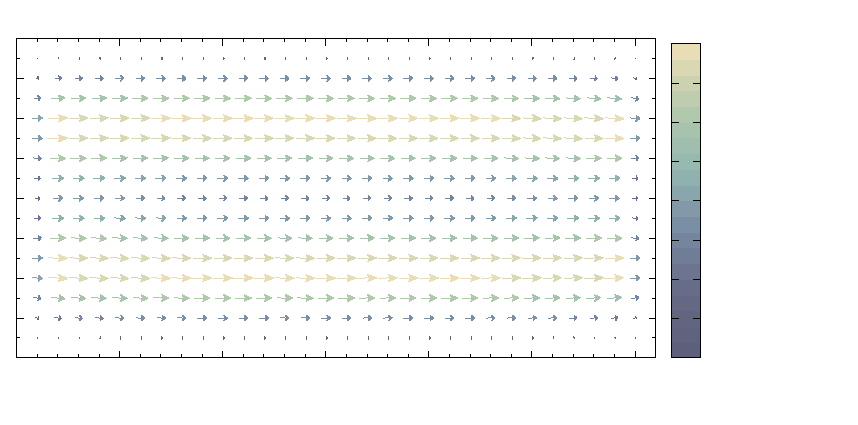
\includegraphics[width={396.00bp},height={188.60bp}]{../Plots/SC30/NotFourier/Currents/FixedLinearPhaseGradient/Phase117deg/mu-3.75/plot}}%
    \gplfronttext
  \end{picture}%
\endgroup

